\chapter{Koncepció}

\section{Mi a Docker?}

A \textbf{Docker} egy nyílt forráskódú platform, amely lehetővé teszi az alkalmazások konténerizálását. A konténerizálás azt jelenti, hogy az alkalmazásokat, azok függőségeit és konfigurációit egyetlen, hordozható konténerbe csomagolja. A Docker konténerek olyan elszigetelt környezeteket biztosítanak, amelyek tartalmazzák az alkalmazás összes szükséges összetevőjét: operációs rendszert, könyvtárakat, függőségeket és magát az alkalmazást is. Így biztosítva van, hogy az alkalmazás ugyanúgy működjön fejlesztői, tesztelői és éles környezetben is, függetlenül attól, hogy az adott környezet milyen operációs rendszert használ vagy milyen egyéb programozási környezetet igényel.

A Docker konténerek előnyei közé tartozik a \textbf{hordozhatóság}, \textbf{skálázhatóság} és az \textbf{elkülönítés}, melyek lehetővé teszik a fejlesztés, tesztelés és üzemeltetés hatékony és zökkenőmentes végrehajtását. A konténerek gyors indítási és leállítási idejei is rendkívül előnyösek, szemben a hagyományos virtuális gépekkel, amelyek nagyobb erőforrást igényelnek és hosszabb ideig tartanak a beállítások és az indítások. 

A Docker konténerek \textbf{elkülönítése} biztosítja, hogy az egyes alkalmazások ne befolyásolják egymást, mivel minden konténer egy saját, független környezetben fut. Ez különösen fontos a mikroszolgáltatások architektúrájában, ahol sok kis, különálló szolgáltatás együttműködik, és ha valamelyik szolgáltatás hibázik, nem befolyásolja a többi működését.

A \textbf{hordozhatóság} lehetővé teszi, hogy ugyanaz a konténer bárhol futtatható legyen, legyen szó helyi gépről, tesztkörnyezetről vagy éles környezetről, különböző operációs rendszereken (Linux, macOS, Windows). A Docker által biztosított \textbf{skálázhatóság} azt jelenti, hogy az alkalmazásokat könnyen és gyorsan bővíthetjük több konténerre, amelyeket automatikusan eloszthatunk különböző szerverek között, optimalizálva a rendszer teljesítményét.

A Docker megoldásainak különösen nagy előnyei vannak a fejlesztők és az üzemeltetők számára. A fejlesztők számára lehetővé teszi, hogy pontosan ugyanazt a környezetet használják minden fázisban (fejlesztés, tesztelés, élesítés), míg az üzemeltetők számára a konténerek biztosítják a könnyű telepítést és frissítést anélkül, hogy a rendszer többi részét befolyásolnák.

A Docker alapú környezetek általában gyorsabbak és erőforráshatékonyabbak, mint a hagyományos virtuális gépek, mivel a Docker nem emulálja az egész operációs rendszert, hanem közvetlenül a gazda operációs rendszer kernelét használja. Ezen kívül a Docker segítségével könnyen létrehozhatók új, azonnal használható fejlesztési és tesztkörnyezetek, ami gyorsítja az alkalmazások fejlesztését és szállítását.

A Docker egyik legfontosabb előnye, hogy lehetővé teszi a konténerek gyors elindítását és leállítását. Mivel a konténerek nem tartalmaznak teljes operációs rendszert, ezért kevesebb erőforrást igényelnek, és gyorsan újraindíthatók. Ez különösen fontos a folyamatos integrációs (CI) és folyamatos szállítási (CD) rendszerekben, ahol a gyors alkalmazás- és környezetbeállítások szükségesek.

\textbf{Docker Compose} eszközzel pedig könnyen kezelhetjük több konténerből álló alkalmazásokat, definiálhatjuk a konténerek közötti kapcsolatokat és beállíthatjuk a szükséges környezetváltozókat, fájlokat és hálózati beállításokat. Ezzel a megoldással képesek vagyunk teljes alkalmazásokat futtatni több különálló konténerben, mint például egy webalkalmazást egy adatbázissal, anélkül, hogy bonyolult konfigurációkat kellene kezelni.

\section{A virtualizáció}
A virtualizáció olyan technológia, amely lehetővé teszi a számítógépes erőforrások, mint a processzor, memória, tároló és hálózati eszközök hatékony kihasználását és szétosztását több független környezet között. A virtualizáció révén egyetlen fizikai gépen több virtuális gép (VM) vagy konténer futhat, amelyek külön operációs rendszert és alkalmazásokat is futtathatnak. A virtualizáció alapvetően két fő típust ölel fel: az 1. típusú (bare-metal) és a 2. típusú (hosted) virtualizációt. Ezen kívül létezik a konténer-alapú virtualizáció, amely a Docker révén vált népszerűvé.


\textbf{1. Típusú virtualizáció (Bare-metal virtualizáció)}: A 1. típusú virtualizáció esetén a virtualizációs szoftver közvetlenül a fizikai hardveren fut, és nem szükséges egy operációs rendszer a futtatásához. Ezáltal a virtualizációs réteg közvetlen hozzáférést biztosít a hardverhez, így jobb teljesítményt és hatékonyabb erőforrás-kihasználást kínál. A 1. típusú virtualizációhoz tartozó rendszerek például a VMware ESXi, Microsoft Hyper-V vagy Xen.

\textbf{2. Típusú virtualizáció (Hosted virtualizáció)}: A 2. típusú virtualizáció egy operációs rendszeren belül futó virtualizációs réteget használ. Ez azt jelenti, hogy a virtualizációs szoftver egy meglévő operációs rendszer (pl. Linux vagy Windows) felett működik, és az operációs rendszer biztosítja az erőforrásokat a virtualizációs réteg számára. Bár a 2. típusú virtualizáció könnyebben beállítható és rugalmasabb, a teljesítménye általában alacsonyabb, mint az 1. típusú virtualizációé. Ilyen példák a VMware Workstation, Oracle VirtualBox vagy Parallels Desktop.

\textbf{Docker és a virtualizáció}: A Docker a konténer-alapú virtualizációt képviseli, amely eltér a hagyományos 1. és 2. típusú virtualizációtól. A Docker konténerek az operációs rendszeren belül, annak erőforrásait használva futnak, de nem igényelnek teljes virtuális gépet, így sokkal könnyebbek és gyorsabbak. A Docker lehetővé teszi a különböző alkalmazások izolálását ugyanazon operációs rendszer keretein belül, de anélkül, hogy teljes virtuális gépeket kellene futtatni. Ez a megoldás ideális a mikroszolgáltatások, DevOps és folyamatos integrációs (CI) rendszerek számára.

\newpage
\section{Docker alapfogalmak}

A Docker alapfogalmai közé tartoznak a következők:

\begin{itemize}
	\item \textbf{Docker Image}: A Docker image egy statikus sablon, amely tartalmazza az alkalmazás futtatásához szükséges összes összetevőt. Az image-ek lehetővé teszik az alkalmazás egyszerű másolását, más környezetekbe történő telepítését.
	\item \textbf{Docker Container}: A konténer az image dinamikus példánya, amely fut a rendszerben. Mivel a Docker image-ek csak a szükséges fájlokat tartalmazzák, a konténer gyorsan elindítható és leállítható.
	\item \textbf{Dockerfile}: A Dockerfile egy szöveges fájl, amely tartalmazza azokat az utasításokat, amelyek meghatározzák, hogy egy Docker image hogyan épül fel. Például egy Dockerfile tartalmazhatja az operációs rendszer választását, a szükséges könyvtárak telepítését, valamint az alkalmazás futtatásához szükséges parancsokat.
	\item \textbf{Docker Compose}: A Docker Compose lehetővé teszi több konténer egyidejű futtatását. Ezzel könnyen kezelhetjük a komplex alkalmazásokat, amelyek több szolgáltatást igényelnek, például adatbázist és webes alkalmazást.
\end{itemize}

\section{Docker használati előnyök}

A Docker legfontosabb előnyei közé tartozik:

\begin{itemize}
	\item \textbf{Hordozhatóság}: A Docker konténerek lehetővé teszik, hogy ugyanazt az alkalmazást futtassuk bármely fejlesztői, tesztelői vagy éles környezetben, függetlenül az operációs rendszertől.
	\item \textbf{Izoláció}: Mivel minden alkalmazás egy saját, izolált konténerben fut, a különböző alkalmazások nem zavarják egymást.
	\item \textbf{Skálázhatóság}: A Docker könnyen integrálható a különböző konténer-orientált orkhesztrációs platformokkal, mint a \textbf{Kubernetes}, lehetővé téve a skálázható alkalmazások létrehozását.
\end{itemize}

\section{Docker parancssoros interfész (CLI)}

A Docker parancssoros interfésze (CLI) az egyik legfontosabb eszköz a Docker környezetek kezelésében. A CLI segítségével a felhasználók közvetlenül kommunikálhatnak a Docker Daemon-nal, amely az alkalmazásokat futtató alaprendszert kezeli. A CLI lehetővé teszi a Docker konténerek, képek, hálózatok, valamint a rendszer konfigurációjának kezelését, mindezt egy egyszerű, szöveges felületen keresztül.

A parancssoros interfész az egyik leghatékonyabb módja annak, hogy automatizáljuk a különböző Docker műveleteket, és integráljuk azokat különböző fejlesztői és üzemeltetési munkafolyamatokba. A Docker CLI segítségével számos olyan műveletet végezhetünk el, mint például a konténerek indítása, leállítása, naplózása, a tárolóeszközök kezelése, valamint a futó konténerek monitorozása.

A leggyakrabban használt CLI parancsok közé tartozik:

\begin{itemize}
	\item \texttt{docker run}: Konténer indítása egy adott image-ből.
	\item \texttt{docker ps}: A futó konténerek listázása.
	\item \texttt{docker build}: Az image-ek létrehozása egy Dockerfile segítségével.
	\item \texttt{docker exec}: Parancs futtatása egy már futó konténerben.
	\item \texttt{docker stop} és \texttt{docker rm}: Konténerek leállítása és eltávolítása.
	\item \texttt{docker logs}: A konténer naplóinak megtekintése.
\end{itemize}

A CLI előnye, hogy közvetlen és gyors hozzáférést biztosít minden Docker erőforráshoz, és lehetővé teszi a különböző műveletek scriptelését is, ami különösen fontos az automatizált környezetekben.

\section{Felügyeleti eszközök}

A Docker környezetek és konténerek kezelése összetett feladat lehet, különösen nagyobb rendszerek esetén, ahol sok konténer fut párhuzamosan. A felügyeleti eszközök célja, hogy egyszerűsítsék a konténerek és alkalmazások kezelését, lehetővé téve azok zökkenőmentes működését. A felügyeleti eszközök biztosítják a szükséges erőforrásokat a konténerek telepítésére, frissítésére és skálázására, emellett biztosítják a folyamatos figyelemmel kísérést és hibaelhárítást.

A Docker konténerek kezelésére számos felügyeleti eszköz létezik, ezek közül a legfontosabbak:

\begin{itemize}
	\item \textbf{Portainer}: A Portainer egy könnyen használható webes felületet kínál a Docker környezetek kezelésére. Lehetővé teszi a felhasználók számára, hogy vizuálisan kezeljék a konténereket, image-eket, hálózatokat és volumeneket, egyszerűsíti a konténerek telepítését, frissítését és leállítását. A Portainer az egyik legnépszerűbb eszköz a Docker rendszergazdák körében, mivel intuitív és egyszerűen használható.
	\item \textbf{Rancher}: A Rancher egy teljes körű platform, amely a konténerek kezelésére és orkhesztrálására szolgál. A Rancher különösen hasznos nagyobb, mikroszolgáltatásokon alapuló alkalmazások esetén, ahol több konténer is fut egyszerre. Az eszköz egy egységes kezelőfelületet kínál a Docker és Kubernetes környezetek számára.
	\item \textbf{Docker Swarm}: A Docker Swarm a Docker által biztosított orkhesztrációs eszköz, amely lehetővé teszi, hogy több konténert egyszerre kezeljünk és eloszlassuk őket több gépen. A Swarm automatikusan képes skálázni a konténerek számát, és biztosítja a konténerek közötti kommunikációt és magas rendelkezésre állást.
	\item \textbf{Kubernetes}: A Kubernetes egy nyílt forráskódú orkhesztrációs platform, amely széleskörű eszközkészletet kínál a konténerek kezelésére. A Kubernetes lehetővé teszi a konténerek automatikus elhelyezését, skálázását, frissítését és monitorozását, amely ideális nagyobb és komplex rendszerekhez.
\end{itemize}

Ezek az eszközök nemcsak a Docker környezetek kezelésére szolgálnak, hanem biztosítják az alkalmazások folyamatos működését és skálázódását is, amely alapvetően fontos a modern fejlesztési és üzemeltetési környezetekben.

\section{Monitorozó eszközök}

A Docker környezetek és konténerek monitorozása alapvetően fontos a teljesítmény és az alkalmazások stabilitásának biztosításához. A monitorozó eszközök segítségével folyamatosan figyelemmel kísérhetjük a konténerek erőforrás-használatát, az alkalmazások válaszidejét, a hálózati forgalmat, valamint a hibaüzeneteket. A hatékony monitorozás segíthet megelőzni a rendszerhibákat, és gyorsan észlelni a teljesítménybeli problémákat.

A legnépszerűbb Docker monitorozó eszközök közé tartoznak:

\begin{itemize}
	\item \textbf{Prometheus}: A Prometheus egy nyílt forráskódú monitorozó és riasztó rendszer, amely különösen a konténerizált környezetekben népszerű. A Prometheus képes gyűjteni és tárolni az alkalmazások és konténerek metrikáit, mint például a CPU-használatot, a memóriahasználatot és a hálózati forgalmat. Az adatok időalapú adatbázisban tárolódnak, és a Grafana segítségével vizualizálhatók.
	\item \textbf{Grafana}: A Grafana egy vizualizációs eszköz, amely a Prometheus által gyűjtött adatokat interaktív és dinamikus grafikonokon jeleníti meg. A Grafana segíti a rendszergazdákat abban, hogy gyorsan észleljék a problémákat, és könnyen azonosíthassák a teljesítménybeli anomáliákat.
	\item \textbf{cAdvisor}: A cAdvisor (Container Advisor) egy Google által kifejlesztett eszköz, amely a Docker konténerek erőforrás-használatát monitorozza. A cAdvisor képes figyelni a CPU-, memória-, hálózati- és lemezhasználatot, és az adatokat a webes felületen jeleníti meg.
	\item \textbf{Datadog}: A Datadog egy felhőalapú monitorozó platform, amely lehetővé teszi a Docker környezetek valós idejű monitorozását. A Datadog integrálódik a Docker és más konténer-orientált rendszerekhez, és automatikusan összegyűjti a rendszer metrikáit, naplóit és egyéb adatokat. A Datadog által kínált riasztások és vizualizációs lehetőségek segítenek a rendszergazdáknak a gyors hibaelhárításban.
\end{itemize}

A monitorozó eszközök folyamatos figyelemmel kísérést biztosítanak, amely lehetővé teszi a gyors reagálást a rendszerproblémákra. A megfelelő monitorozás segít a Docker környezetek optimalizálásában és a teljesítmény folyamatos javításában.


\section{A Docker Manager és a projekt technológiai háttere}

Az alkalmazásom célja, hogy leegyszerűsítse a Docker konténerek kezelését egy felhasználóbarát grafikus felületen keresztül. A Docker, mint egyre népszerűbb eszköz az alkalmazások konténerizálására, sok fejlesztő számára kínál megoldásokat, azonban a parancssoros kezelés nem mindenki számára intuitív. A DockerManager ezt a problémát orvosolja azáltal, hogy lehetővé teszi a felhasználók számára a konténerek kezelését, anélkül, hogy parancssoros utasításokat kellene adniuk.

A projekt Python nyelven készült, mivel a Python egy rendkívül rugalmas és széles körben használt nyelv, amely tökéletes választás a gyors fejlesztéshez és az alkalmazások szoros integrálásához különböző rendszerekkel. A grafikus felület fejlesztéséhez a \textbf{PyQt5} könyvtárat választottam, mivel az egy jól dokumentált, stabil, és keresett eszköz a Python számára a GUI (grafikus felhasználói felület) létrehozásához. A PyQt5 lehetővé teszi, hogy gyorsan és hatékonyan hozzunk létre asztali alkalmazásokat, miközben teljes mértékben kihasználjuk a Qt keretrendszer erejét és funkcionalitását, amely egyesíti az esztétikai szempontokat és a könnyű használhatóságot.

Az alkalmazás lehetőséget biztosít a felhasználók számára a Docker konténerek egyszerű kezelésére. Az alkalmazás grafikus felületén keresztül a felhasználók képesek:
\begin{itemize}
	\item \textbf{Konténerek indítása}: Az alkalmazás lehetővé teszi a konténerek gyors indítását anélkül, hogy a felhasználóknak parancsokat kellene futtatniuk. A felhasználó egyszerűen kiválaszthatja a kívánt Docker image-et, és az alkalmazás automatikusan elindítja a konténert a háttérben.
	\item \textbf{Konténerek leállítása}: A konténerek leállítása is egyszerűen elvégezhető a grafikus felületen, egyetlen kattintással. A felhasználónak nem kell aggódnia a parancssori utasítások helyességéről, hiszen a folyamatot teljes mértékben automatizálja az alkalmazás.
	\item \textbf{Monitorozás és kezelés}: Az alkalmazás képes nyújtani valós idejű információkat a futó konténerek állapotáról, beleértve a CPU és memória használatot, a hálózati forgalmat, valamint a konténerek logjait. A felhasználók egyszerűen átvizsgálhatják a konténereket a kezelőfelületen, és szükség esetén elvégezhetik a megfelelő beállításokat.
	\item \textbf{Képek kezelése}: A Docker képek kezelése szintén elérhető az alkalmazáson keresztül, így a felhasználók könnyen telepíthetnek új képeket, törölhetik a feleslegeseket vagy akár frissíthetik a meglévő képeket.
\end{itemize}

Célja, hogy egy könnyen kezelhető, vizuális interfészt biztosítson, amely jelentősen csökkenti a Docker kezelésére fordított időt és bonyolultságot, különösen azok számára, akik nem rendelkeznek mélyebb parancssoros ismeretekkel.

A program a Docker Engine API-jával kommunikál a háttérben, amely biztosítja a konténerek és képek kezelését. A felhasználói interakciók az alkalmazás grafikus felületén keresztül valósulnak meg, miközben az alkalmazás a Python docker könyvtárát használja a Docker parancsok végrehajtásához. Ez a megoldás lehetővé teszi, hogy az alkalmazás egyszerűsítse a komplex Docker műveleteket anélkül, hogy a felhasználóknak közvetlenül kellene parancsokat futtatniuk.

Az alkalmazás tehát nemcsak kezdő felhasználók számára biztosít könnyen használható eszközt, hanem a haladó Docker felhasználók számára is lehetőséget ad arra, hogy gyorsabban végezzenek el rutinfeladatokat, például a konténerek indítását vagy leállítását. Az \texttt{DockerManager} egy egyszerű, de hatékony eszközzé válik mindenki számára, aki Docker környezetben dolgozik, és akik a konténerek kezelését egy vizuális, felhasználóbarát eszközzel kívánják végezni.

Az alkalmazás további előnye, hogy könnyen bővíthető és testreszabható, így új funkciók, például a konténer állapotok részletesebb monitorozása vagy a hálózati beállítások kezelése, könnyen integrálhatók a jövőbeni fejlesztések során.

\section{Hasonló célú alkalmazások }

A Docker környezetek kezelése során számos grafikus és parancssori eszköz közül választhatunk. Ezek az eszközök különféle funkciókat kínálnak a konténerek létrehozásához, konfigurálásához, monitorozásához és menedzseléséhez.

\subsection{Docker Desktop}
\begin{figure}[H]
	\centering
	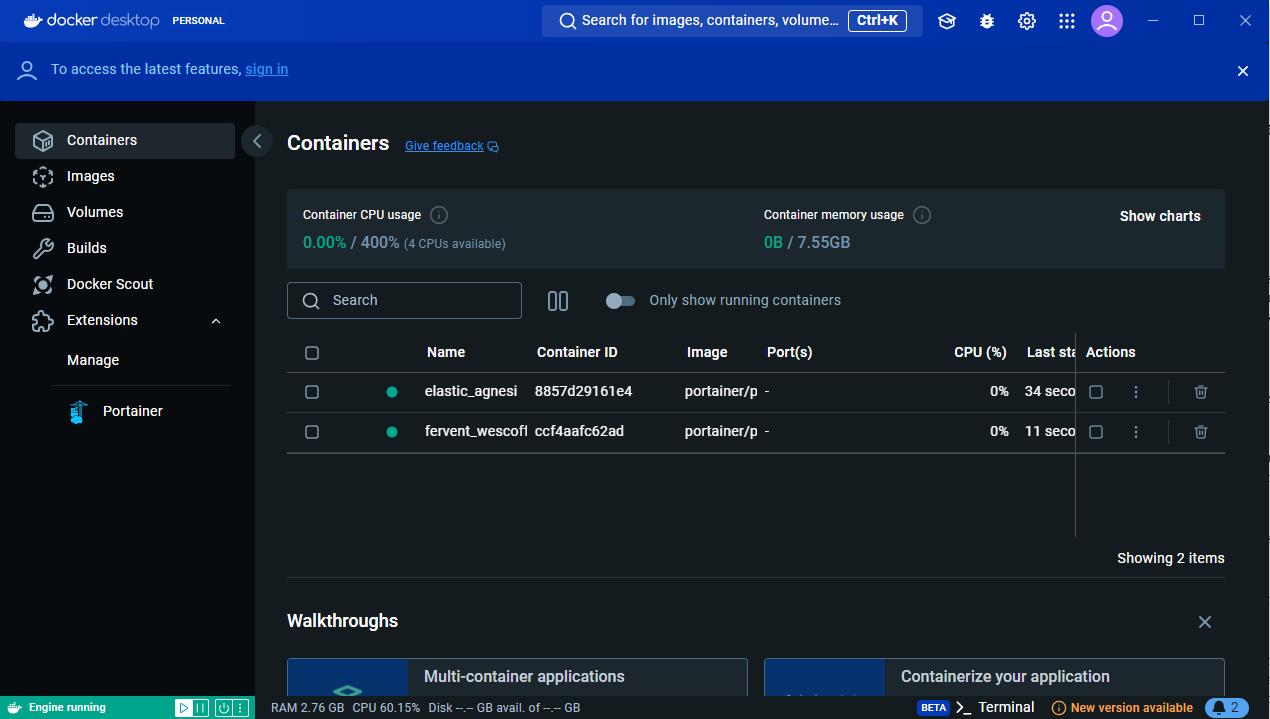
\includegraphics[width=0.7\linewidth]{images/Docker_desktop}
	\caption{Docker Desktop}
	\label{fig:dockerdesktop}
\end{figure}


A \textbf{Docker Desktop} egy hivatalos Docker termék, amely Windows és macOS rendszerekre készült (nemrégiben pedig Linuxra is elérhetővé vált), és célja, hogy a fejlesztők könnyen kezelhessék a helyi konténereket anélkül, hogy bonyolult telepítési folyamatokon kellene keresztülmenniük. A Docker Desktop képes a konténerizált alkalmazások gyors és egyszerű telepítésére, indítására és kezelésére.

\textbf{Fő funkciók}:
\begin{itemize}
	\item \textbf{Helyi fejlesztési környezet}: Lehetővé teszi fejlesztési és tesztelési környezetek gyors kialakítását és futtatását helyi gépeken.
	\item \textbf{Kubernetes támogatás}: A Docker Desktop beépített Kubernetes klasztert biztosít, így a fejlesztők tesztelhetik és konfigurálhatják Kubernetes-be telepítendő alkalmazásaikat helyi környezetben.
	\item \textbf{Integrált Docker CLI}: A parancssori felület használatával kombinálva az eszköz rugalmasságot kínál mind a kezdő, mind a haladó felhasználók számára.
	\item \textbf{Docker Compose támogatás}: Az összetettebb alkalmazások Docker Compose segítségével való kezelésére is alkalmas.
\end{itemize}

\textbf{Alkalmazási területek}:
A Docker Desktop kiváló megoldás fejlesztők számára, akik egyszerűen szeretnének lokális Docker környezetet használni. Hasznos lehet kisebb tesztelési feladatokra, valamint olyan fejlesztési folyamatokhoz, ahol Kubernetes környezetre is szükség van.

\subsection{Portainer}

\begin{figure}[H]
	\centering
	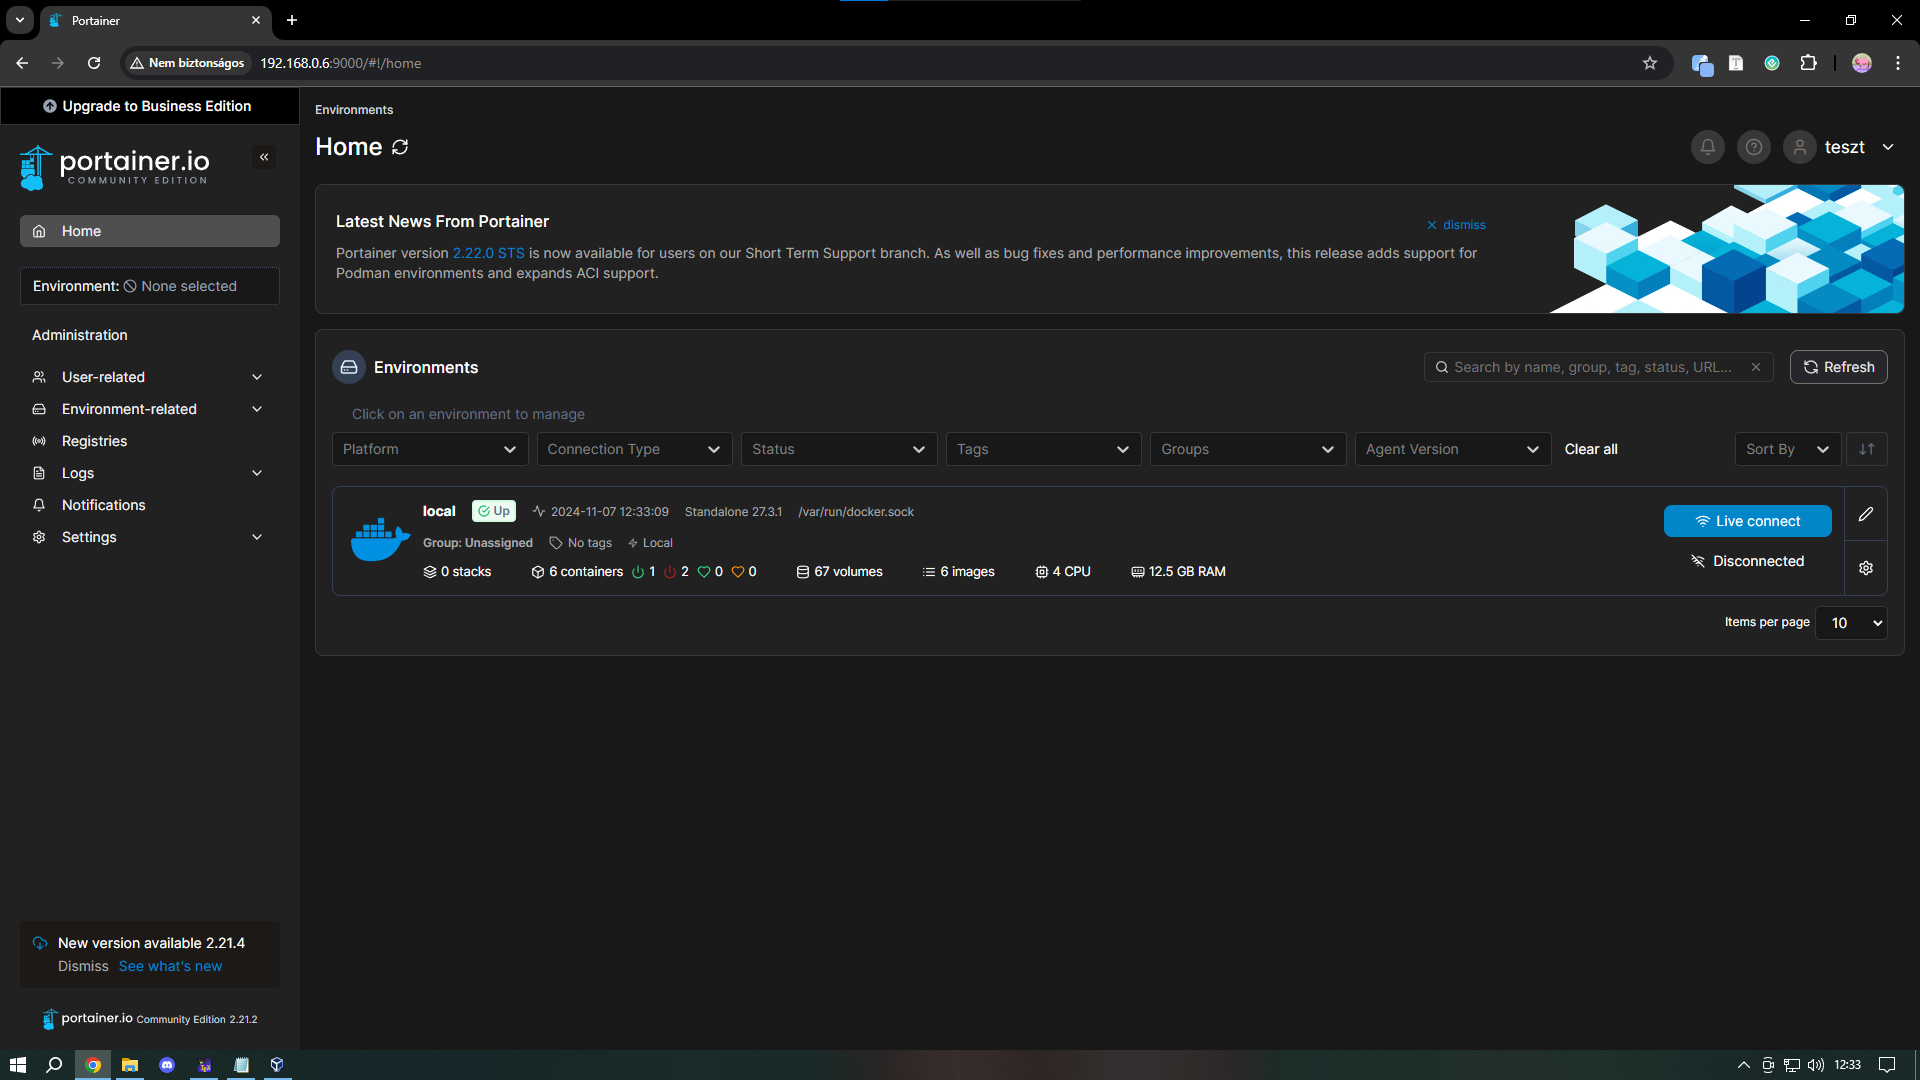
\includegraphics[width=0.7\linewidth]{images/portainer}
	\caption{Portainer}
	\label{fig:portainer}
\end{figure}


A \textbf{Portainer} egy nyílt forráskódú, webalapú menedzsment eszköz, amely platformfüggetlen módon képes kezelni a Docker és Kubernetes környezeteket. Könnyű felhasználói felületének köszönhetően különösen népszerű választás a DevOps szakemberek körében.

\textbf{Fő funkciók}:
\begin{itemize}
	\item \textbf{Webes menedzsment felület}: Felhasználóbarát felület, amely lehetővé teszi a konténerek, képek és hálózatok kezelését böngészőből.
	\item \textbf{Integráció Docker Swarm és Kubernetes támogatással}: Nagyobb környezetek és klaszterek kezelésére is alkalmas.
	\item \textbf{Részletes felügyelet és monitorozás}: CPU és memória használati adatok figyelése, valamint a konténerek állapotának követése.
	\item \textbf{Role-based access control (RBAC)}: Felhasználói jogosultságok beállítása a nagyobb szervezeti használatra.
\end{itemize}

\textbf{Alkalmazási területek}:
A Portainer elsősorban rendszergazdák és DevOps szakemberek számára készült, akik egyszerűsített, webes felületen szeretnék kezelni és felügyelni a konténerek működését, különösen nagyobb, elosztott rendszerekben vagy Kubernetes környezetekben.

\subsection{Rancher}

\begin{figure}[H]
	\centering
	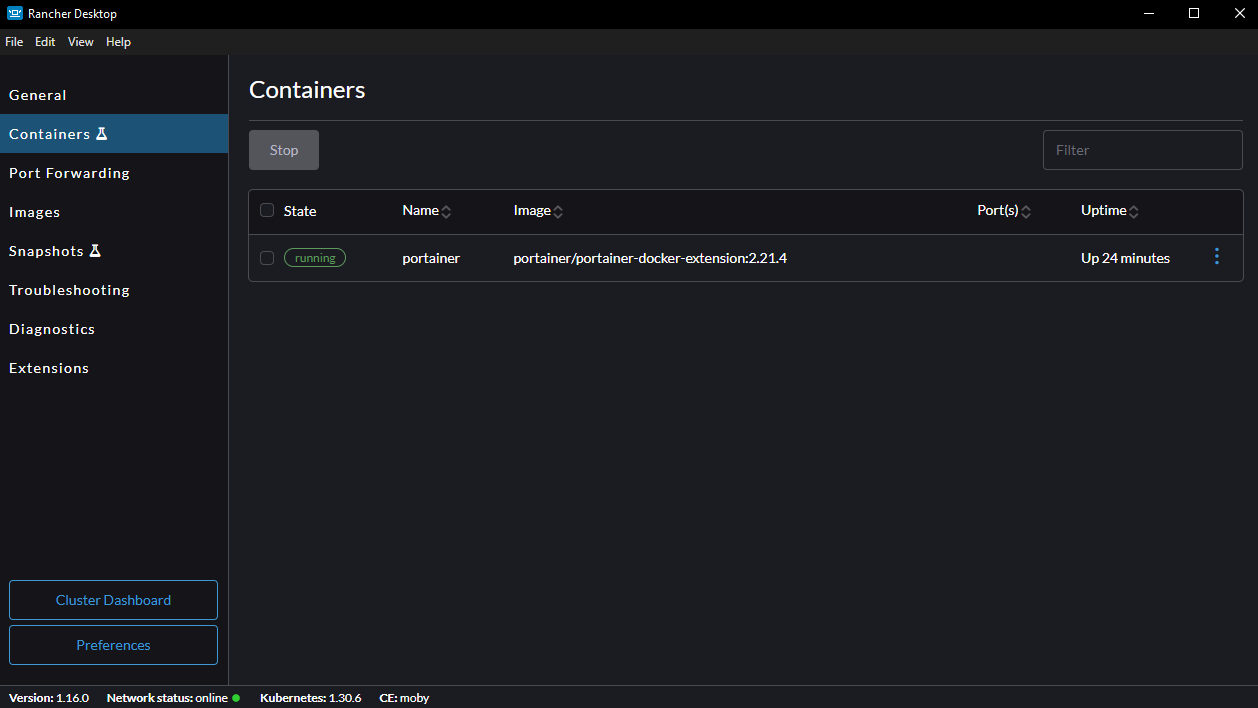
\includegraphics[width=0.7\linewidth]{images/rancher}
	\caption{Rancher Desktop}
	\label{fig:rancher}
\end{figure}


A \textbf{Rancher} egy Kubernetes menedzsment platform, amely támogatja a több klaszteres Kubernetes környezetek kezelését és monitorozását. Ez az eszköz célzottan Kubernetes-re optimalizált, és széles körben használják olyan vállalatok, amelyek Kubernetes alapú infrastruktúrát használnak.

\textbf{Fő funkciók}:
\begin{itemize}
	\item \textbf{Kubernetes klaszterek kezelése és skálázása}: Egyszerűen kezelhetők és monitorozhatók több klaszteres Kubernetes környezetek.
	\item \textbf{CI/CD támogatás}: Beépített támogatás folyamatos integrációhoz és telepítéshez, amely GitHub és más CI/CD eszközökkel együttműködik.
	\item \textbf{Többfelhős támogatás}: Alkalmazkodik különféle felhőszolgáltatásokhoz (AWS, GCP, Azure), így többféle környezetet kezelhet egy helyen.
	\item \textbf{API és plugin támogatás}: Számos külső eszközzel és alkalmazással integrálható.
\end{itemize}

\textbf{Alkalmazási területek}:
A Rancher ideális választás olyan nagyobb vállalatok számára, amelyek Kubernetes alapú infrastruktúrát használnak, és szükségük van egy robusztus eszközre, amely biztosítja a konténerizált alkalmazások skálázhatóságát és integrálhatóságát több klaszterben is.

\subsubsection{A Kubernetes}

A \textbf{Kubernetes} (gyakran rövidítve K8s) egy nyílt forráskódú konténer-orchestration eszköz, amelyet eredetileg a Google fejlesztett ki, és amelyet jelenleg a Cloud Native Computing Foundation (CNCF) támogat. Célja a konténerizált alkalmazások automatizált üzemeltetése, beleértve azok telepítését, skálázását és kezelését. Mivel a modern alkalmazások gyakran mikroszolgáltatásokon alapulnak, és egyre inkább konténerizált környezetben futnak, a Kubernetes kulcsfontosságú eszközzé vált a nagyvállalati és felhőalapú infrastruktúrában.

\subsubsection{Kubernetes fő komponensei}

A Kubernetes rendszere több összetevőből áll, amelyek együttesen biztosítják a konténerek kezelését és az erőforrások optimális elosztását:

\begin{itemize}
	\item \textbf{Node-ok és Pod-ok}: A Kubernetes a konténereket úgynevezett \textbf{Pod}-okban futtatja, amelyek a legkisebb telepíthető egységek. Minden pod egy vagy több konténert tartalmaz, amelyek közös hálózati környezetben és fájlrendszeren osztoznak. A \textbf{node-ok} azok a gépek (virtuális vagy fizikai szerverek), amelyek a pod-okat futtatják.
	
	\item \textbf{Master komponensek}: A \textbf{master} a Kubernetes központi komponense, amely irányítja a cluster működését. A legfontosabb master komponensek:
	\begin{itemize}
		\item \textbf{API Server}: Kommunikációs interfészként szolgál a felhasználók és a Kubernetes többi része között.
		\item \textbf{Controller Manager}: Figyeli a cluster állapotát, és végrehajtja az olyan szabályozási feladatokat, mint a skálázás vagy a pod-ok helyreállítása.
		\item \textbf{Scheduler}: Felelős a pod-ok elhelyezéséért a node-okon, optimalizálva a rendelkezésre álló erőforrásokat.
	\end{itemize}
	
	\item \textbf{Kubelet}: Minden node-on egy \textbf{kubelet} nevű ügynök fut, amely biztosítja, hogy a node-ok ténylegesen a kívánt pod-okat futtassák.
\end{itemize}

\subsubsection{Kubernetes előnyei}

A Kubernetes népszerűsége számos előnyének köszönhető:

\begin{itemize}
	\item \textbf{Automatizált telepítés és skálázás}: A Kubernetes lehetővé teszi a konténerek automatikus telepítését, skálázását és újraindítását, így nagy mennyiségű alkalmazás könnyedén futtatható elosztott környezetekben.
	\item \textbf{Öngyógyító képesség}: Ha egy konténer meghibásodik, a Kubernetes automatikusan újraindítja vagy áthelyezi, biztosítva az alkalmazások magas rendelkezésre állását.
	\item \textbf{Deklaratív konfiguráció}: A Kubernetes deklaratív megközelítést használ, lehetővé téve a rendszergazdák számára, hogy az állapotot konfigurációs fájlokban határozzák meg, a rendszer pedig automatikusan megpróbálja elérni ezt az állapotot.
\end{itemize}

\subsubsection{Docker és Kubernetes kapcsolata}

Bár a Kubernetes képes különböző konténer futtatómotorokkal működni, hagyományosan a Docker konténerekkel együtt használják, mivel mindkét technológia célja a modern, mikroszolgáltatás-alapú architektúrák támogatása. A Kubernetes segítségével a Docker konténerek kezelése sokkal skálázhatóbb és automatizáltabb, amely különösen hasznos komplex rendszerek és mikroszolgáltatás-architektúrák esetében.


\subsection{LazyDocker}

\begin{figure}[H]
	\centering
	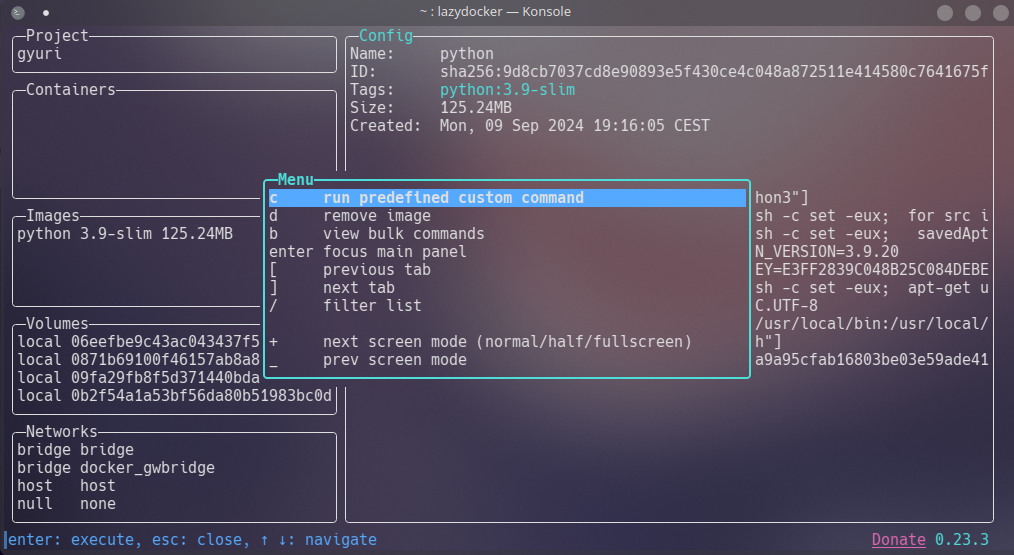
\includegraphics[width=0.7\linewidth]{images/lazydocker}
	\caption[]{Lazydocker}
	\label{fig:lazydocker}
\end{figure}

A \textbf{LazyDocker} egy minimalista, terminál-alapú felületet kínál, amely a Docker CLI használatát egyszerűsíti. Bár nem nyújt grafikus felületet, vizuálisan átlátható módon jeleníti meg a parancssori felületen elérhető funkciókat, és célja a Docker-rel dolgozó fejlesztők munkájának egyszerűsítése.



\textbf{Fő funkciók}:
\begin{itemize}
	\item \textbf{Konténerek és képek kezelése}: Gyors parancsokat biztosít a konténerek indításához, leállításához, újraindításához, valamint a képek kezeléséhez.
	\item \textbf{Log monitorozás}: Részletes log megjelenítés a hibakereséshez és a konténerek állapotának követéséhez.
	\item \textbf{Képernyőn megjelenített statisztikák}: Valós idejű CPU és memória használati adatok jelennek meg, ami segíti az erőforrás-kihasználtság nyomon követését.
\end{itemize}

\textbf{Alkalmazási területek}:
A LazyDocker hasznos eszköz fejlesztők számára, akik parancssori környezetben dolgoznak, és vizuálisan is átláthatóbbá szeretnék tenni a Docker parancsokat. Ideális kisebb fejlesztési környezetekben, ahol gyorsan szükséges kezelni a konténereket és erőforrás-felhasználási statisztikákat.